\documentclass[a4paper]{article}

\usepackage[UTF8]{ctex}
\usepackage{ReportTemplate}

\usepackage{setspace}
\usepackage{amsmath}
\usepackage{algorithm}
\usepackage{algpseudocode}
\usepackage[hidelinks]{hyperref}

\setmainfont{Times New Roman}
\newcommand{\best}[1]{\textbf{#1}}
\floatname{algorithm}{算法}
\renewcommand{\algorithmicrequire}{\textbf{输入:}}
\renewcommand{\algorithmicensure}{\textbf{输出:}}

\title{Project 1：语音端点检测}
\name{李颢辰}
\studentid{523030910243}

\begin{document}

\maketitle

\section{问题分析与符号定义}

语音端点检测的目标是在给定语音序列中判定每一帧是否属于语音。设离散语音信号为
$x[n], n=0,\dots,N-1$，采样率记为 $f_s=16$ kHz。所有实验统一采用帧长
$T_w=32$ ms、帧移 $T_h=8$ ms，与标签生成规则保持一致。

\subsection{问题表述}

设每帧长度和帧移对应的采样点数分别为
$L=\mathrm{round}(f_s T_w)$、$H=\mathrm{round}(f_s T_h)$。第 $t$ 帧信号记为
\begin{equation}
  \vec{x}_t = [x[tH],x[tH+1],\dots,x[tH+L-1]]^\top \in \mathbb{R}^{L},
\end{equation}
并乘以窗函数 $w[\cdot]$ 得到分析帧
\begin{equation}
  \tilde{\vec{x}}_t = \vec{x}_t \odot \vec{w}.
\end{equation}
对应的帧级标签记为 $y_t \in \{0,1\}$，其中 $y_t=1$ 表示语音帧，$y_t=0$ 表示非语音帧。
端点检测可统一写为学习如下映射关系：
\begin{equation}
  s_t = f(\vec{f}_t), \qquad \hat{y}_t = g(s_t),
\end{equation}
其中 $\vec{f}_t$ 为第 $t$ 帧特征，$s_t$ 为该帧得分，$\hat{y}_t$ 为最终分类结果。

\subsection{符号定义}
\begin{table}[ht]
  \caption{统一符号定义}
  \label{tab:symbols}
  \centering
  \small
  \begin{tabular}{ll}
    \toprule
    符号 & 含义 \\
    \midrule
    $\vec{x}_t$ & 第 $t$ 帧时域信号 \\
    $\tilde{\vec{x}}_t$ & 加窗后的第 $t$ 帧信号 \\
    $L,H$ & 帧长与帧移对应的采样点数 \\
    $\vec{f}_t$ & 第 $t$ 帧最终特征向量 \\
    $y_t,\hat{y}_t$ & 真实标签与预测标签 \\
    $s_t$ & 语音得分或后验概率 \\
    $\tau,\tau_h,\tau_l$ & 单阈值、双阈值中的高低阈值 \\
    $\mathcal{D}_{\text{tr}},\mathcal{D}_{\text{dev}},\mathcal{D}_{\text{te}}$ & 训练、开发、测试集合 \\
    \bottomrule
  \end{tabular}
\end{table}

\subsection{标签与评测}

数据集原始标签以语音起止时间段给出，实验中先将其转为帧级标签，再与特征帧数对齐；测试阶段则将
帧级预测结果重新转换为时间段输出。因此，模型训练、阈值选择和指标统计均在帧级空间完成。
在数据使用上，Task1 仅在 $\mathcal{D}_{\text{dev}}$ 上进行阈值调整并给出最终结果，
再将同一组参数用于 $\mathcal{D}_{\text{te}}$；Task2 使用 $\mathcal{D}_{\text{tr}}$ 学习
GMM/DNN 模型参数，再在 $\mathcal{D}_{\text{dev}}$ 上进行阈值选择与性能统计，最后在
$\mathcal{D}_{\text{te}}$ 上生成测试结果。

\section{Task1：基于线性分类器和语音短时能量的简单语音端点检测算法}

\subsection{数据预处理及特征提取}

Task1 的处理流程为：分帧、末帧零填充、可选加窗、提取短时特征、逐帧判决。分帧用于把非平稳
语音近似为短时平稳信号；末帧补零保证数据格式对齐，每一帧的长度相等；Hamming 窗可减弱帧
边界处的不连续性，从而降低频谱泄漏。本实验同时比较无窗与 Hamming 窗，并提取四类短时特征组成特征向量
\begin{equation}
  \vec{f}_t^{(1)} = [\bar{E}_t, \bar{Z}_t, \bar{S}_t, \bar{P}_t]^\top.
\end{equation}

\subsubsection{短时能量}
\label{sec:task1-features}

\textbf{概念：}短时能量描述一帧语音波形在短时间内的幅度强弱，是最直接的时域能量统计量。
\textbf{听觉直观：}能量较高的帧通常听起来更响，更可能处在语音主体部分；静音、停顿或背景弱噪声
通常能量较低。\textbf{公式定义：}
\begin{equation}
  E_t = \log \left( \sum_{m=0}^{L-1} \tilde{x}_t^2[m] + \varepsilon \right),
\end{equation}
其中 $\varepsilon$ 为数值稳定项。随后按整段语音做标准化，
\begin{equation}
  \bar{E}_t = \frac{E_t-\mu_E}{\sigma_E+\varepsilon}.
\end{equation}

\subsubsection{过零率}

\textbf{概念：}过零率描述一帧波形穿越零幅度轴的频繁程度，反映信号符号变化的快慢。
\textbf{听觉直观：}过零率较高的片段往往更尖锐或噪声感更强，如摩擦音、清音或部分背景噪声；有声
元音等稳定浊音的过零率通常较低。\textbf{公式定义：}
\begin{equation}
  Z_t = \frac{1}{2(L-1)} \sum_{m=0}^{L-2}
  \left|\operatorname{sgn}(\tilde{x}_t[m+1])-\operatorname{sgn}(\tilde{x}_t[m])\right|.
\end{equation}
\begin{equation}
  \bar{Z}_t = \frac{Z_t-\mu_Z}{\sigma_Z+\varepsilon}.
\end{equation}

\subsubsection{短时频谱}

\textbf{概念：}短时频谱描述一帧信号在不同频率上的幅度分布，本实验使用每帧 log-magnitude 谱均值作
为一维频域统计量。\textbf{听觉直观：}频谱能反映声音的明暗和频率成分分布；语音通常具有较稳定的
频带结构，而静音或部分噪声的频谱形态更分散或更弱。\textbf{公式定义：}设第 $t$ 帧的离散频谱为
\begin{equation}
  X_t[k]=\sum_{m=0}^{L-1}\tilde{x}_t[m]\exp\left(-j2\pi km/L\right),
\end{equation}
则短时频谱统计量定义为
\begin{equation}
  S_t = \frac{1}{K_s}\sum_{k=0}^{K_s-1}\log\left(1+|X_t[k]|\right),
  \qquad
  \bar{S}_t = \frac{S_t-\mu_S}{\sigma_S+\varepsilon}.
\end{equation}

\subsubsection{基频}

\textbf{概念：}基频 $F_0$ 描述有声语音声带周期振动的基本频率，本实验用自相关峰值对应的频率作近似
估计。\textbf{听觉直观：}基频直接对应主观音高；浊音通常具有稳定周期性和较明确的音高，清音、噪
声或静音则往往没有可靠基频。\textbf{公式定义：}先计算帧内自相关
\begin{equation}
  R_t[\ell]=\sum_{m=0}^{L-1-\ell}\tilde{x}_t[m]\tilde{x}_t[m+\ell],
\end{equation}
并在 $f_{\min}=60$ Hz、$f_{\max}=400$ Hz 对应的滞后区间
$\ell\in[\lfloor f_s/f_{\max}\rfloor,\lfloor f_s/f_{\min}\rfloor]$ 内寻找峰值：
\begin{equation}
  \ell_t^\star=\arg\max_{\ell} R_t[\ell].
\end{equation}
\begin{equation}
  P_t=
  \begin{cases}
    f_s/\ell_t^\star, & R_t[\ell_t^\star]/R_t[0]\ge 0.3,\\
    0, & \text{otherwise}.
  \end{cases}
\end{equation}
随后做标准化 $\bar{P}_t=(P_t-\mu_P)/(\sigma_P+\varepsilon)$。

% \textbf{伪代码说明：}以下代码对应 Task1 的短时能量、过零率、短时频谱与基频特征提取流程。

% \begin{lstlisting}[language=python]
% def extract_task1_features(waveform):
%     frames = frame(waveform, win=32ms, hop=8ms, pad=True)
%     frames = hamming_window(frames)
%     energy = log(sum(frames ** 2, axis=1) + eps)
%     energy = (energy - mean(energy)) / (std(energy) + eps) # 能量特征提取
%     zcr = 0.5 * mean(abs(diff(sign(frames), axis=1)), axis=1)
%     zcr = (zcr - mean(zcr)) / (std(zcr) + eps) #过零率特征提取
%     spectrum = mean(log1p(abs(rfft(frames))), axis=1)
%     spectrum = (spectrum - mean(spectrum)) / (std(spectrum) + eps) # 短时频谱特征提取
%     pitch = autocorr_f0(frames, f_min=60, f_max=400, min_ratio=0.3)
%     pitch = (pitch - mean(pitch)) / (std(pitch) + eps) # 基频特征提取
%     return stack([energy, zcr, spectrum, pitch], axis=1)
% \end{lstlisting}

\subsection{算法描述}

\subsubsection{线性打分与双阈值判决}

Task1 的帧级得分写为
\begin{equation}
  s_t 
  = \boldsymbol{\omega}^{\top}
  [\bar{E}_t,-\bar{Z}_t,\bar{S}_t,\bar{P}_t]^{\top}.
\end{equation}
其中 $\boldsymbol{\omega}=[\omega_E,\omega_Z,\omega_S,\omega_P]^\top$ 为可调权重；过零率项取负号，
表示过高的符号变化率更可能对应噪声或非稳定语音。单特征实验可视为仅保留对应权重，组合特征实验
则通过调整多项权重完成。
在此基础上采用双阈值滞回判决，避免单阈值在边界处频繁抖动。记状态变量为 $q_t \in \{0,1\}$，则
\begin{equation}
q_t=
\begin{cases}
1, & s_t>\tau_h \text{ 且 } q_{t-1}=0,\\
0, & s_t<\tau_l \text{ 且 } q_{t-1}=1,\\
q_{t-1}, & \text{其他情况}.
\end{cases}
\end{equation}
最终输出 $\hat{y}_t=q_t$。

阈值 $(\tau_h,\tau_l)$ 在有标签数据上通过网格搜索确定：先在所有帧得分上取若干分位点作为候选集，
再枚举 $\tau_l \le \tau_h$ 的组合，以帧级准确率最高者作为最终参数。Task1 中阈值在
$\mathcal{D}_{\text{dev}}$ 帧级样本上估计，并用于得到 $\mathcal{D}_{\text{dev}}$ 最终结果。
$\mathcal{D}_{\text{dev}}$ 评估阶段对二值输出再做一次长度为 $50$ 的中值平滑，
以削弱孤立误检。

\textbf{伪代码说明：}以下代码对应 Task1 的双阈值滞回判决与中值平滑流程。

\begin{lstlisting}[language=python]
def decode_task1(features, weights, tau_h, tau_l):
    energy, zcr, spectrum, pitch = features.T
    scores = (
        weights.energy * energy
        - weights.zcr * zcr
        + weights.spectrum * spectrum
        + weights.pitch * pitch
    )
    state, pred = 0, []
    for s in scores:
        if state == 0 and s > tau_h:
            state = 1
        elif state == 1 and s < tau_l:
            state = 0
        pred.append(state)
    return median_smooth(pred, kernel=50)
\end{lstlisting}

\subsubsection{测试阶段输出}

\textbf{未知标签端点检测说明：}Task1 测试时不再重新选择阈值，而是复用
$\mathcal{D}_{\text{dev}}$ 上确定的 $(\tau_h,\tau_l)$，对未知标签的测试集语音依次执行分帧、特征提取、双阈值
判决、中值平滑和语音区间合并。

具体地，模型先对未知语音得到逐帧预测 $\hat{y}_t$，再把连续满足 $\hat{y}_t=1$ 的帧合并为一段
语音。若语音段对应帧索引 $a,\dots,b$，则用首尾帧中心时间近似端点，即
$(aH+L/2)/f_s$ 到 $(bH+L/2)/f_s$，最后按 `start,end start,end ...` 的格式输出。

\textbf{伪代码说明：}以下代码对应 Task1 在未知语音上的端点输出流程。

\begin{lstlisting}[language=python]
def infer_task1_unknown(waveform, weights, tau_h, tau_l):
    features = extract_task1_features(waveform)
    pred = decode_task1(features, weights, tau_h, tau_l)
    segments = frames_to_segments(pred, win=32ms, hop=8ms)
    return format_as_label(segments)
\end{lstlisting}

\subsection{实验结果}

\subsubsection{实验指标}

本任务主要从帧级分类质量和阈值相关性能两方面评价模型。所有指标均先将整个 $\mathcal{D}_{\text{dev}}$ 的逐帧预测结果
与逐帧标签拼接，再统一统计。

\begin{itemize}
  \item Accuracy: $\mathrm{Acc}=(TP+TN)/(TP+TN+FP+FN)$，衡量整体判决正确率。
  \item Precision: $\mathrm{Prec}=TP/(TP+FP)$，反映被判为语音的帧中有多少是真语音。
  \item Recall: $\mathrm{Rec}=TP/(TP+FN)$，反映真实语音帧中有多少被正确检出。
  \item $F_1$ score: $F_1=2\mathrm{Prec}\mathrm{Rec}/(\mathrm{Prec}+\mathrm{Rec})$，综合反映精确率与召回率的平衡。
  \item False Acceptance Rate: $\mathrm{FAR}=FP/(FP+TN)$，表示把非语音误判为语音的比例。
  \item False Rejection Rate: $\mathrm{FRR}=FN/(TP+FN)$，表示把语音误判为非语音的比例。
  \item AUC: ROC 曲线下的面积，反映不同阈值下 TPR 与 FAR 的整体表现，越大表示模型整体区分能力越强。
  \item EER: FAR 与 FRR 相等时的错误率，越小越好。
\end{itemize}

\subsubsection{实验配置}

\begin{itemize}
  \item 数据划分：Task1 仅使用 $\mathcal{D}_{\text{dev}}$ 进行权重配置比较、双阈值选择与性能统计，并将同一配置用于未知标签数据推理。
  \item 分帧参数：采样率 $f_s=16$ kHz，帧长 $T_w=32$ ms，帧移 $T_h=8$ ms，因此 $L=512$、$H=128$。
  \item 特征：Task1 尝试使用短时能量，过零率，短时频谱和基频 4 种特征；下方表格中能量\&过零率表示 $\boldsymbol{\omega}=[0.8,0.2,0,0]^\top$，其中过零率以负权进入得分。
  \item 判决与后处理：在 $\mathcal{D}_{\text{dev}}$ 上搜索 $(\tau_h,\tau_l)$，采用双阈值滞回判决，并使用长度为 $50$ 的中值平滑抑制孤立误检。
\end{itemize}

\subsubsection{结果分析}

\begin{center}
  \scriptsize
  \setlength{\tabcolsep}{2.4pt}
  \captionof{table}{Task1 $\mathcal{D}_{\text{dev}}$ 结果（\%）}
  \label{tab:task1-main}
  \resizebox{\columnwidth}{!}{%
    \begin{tabular}{llrrrrrrrr}
      \toprule
      模型特征 & 窗函数 & Acc & Prec & Rec & $F_1$ & FAR & FRR & AUC & EER \\
      \midrule
      能量 & None & \best{95.12} & \best{96.76} & 97.28 & \best{97.02} & \best{14.49} & 2.72 & \best{96.64} & \best{8.34} \\
      能量 & Hamming & 94.45 & 95.85 & 97.43 & 96.63 & 18.80 & 2.57 & 96.17 & 9.09 \\
      过零率 & None & 81.64 & 81.65 & \best{99.98} & 89.89 & 100.00 & \best{0.02} & 56.50 & 41.37 \\
      频谱 & None & 94.00 & 96.50 & 96.14 & 96.32 & 15.52 & 3.86 & 95.04 & 9.99 \\
      基频 & None & 81.67 & 81.79 & 99.76 & 89.89 & 98.85 & 0.24 & 50.33 & 44.69 \\
      能量\&过零率 & None & 93.50 & 94.96 & 97.20 & 96.07 & 22.95 & 2.80 & 95.36 & 10.38 \\
      能量\&过零率 & Hamming & 93.38 & 94.86 & 97.17 & 96.00 & 23.45 & 2.83 & 94.81 & 11.21 \\
      \bottomrule
    \end{tabular}%
  }
\end{center}

\begin{center} 
  \centering
  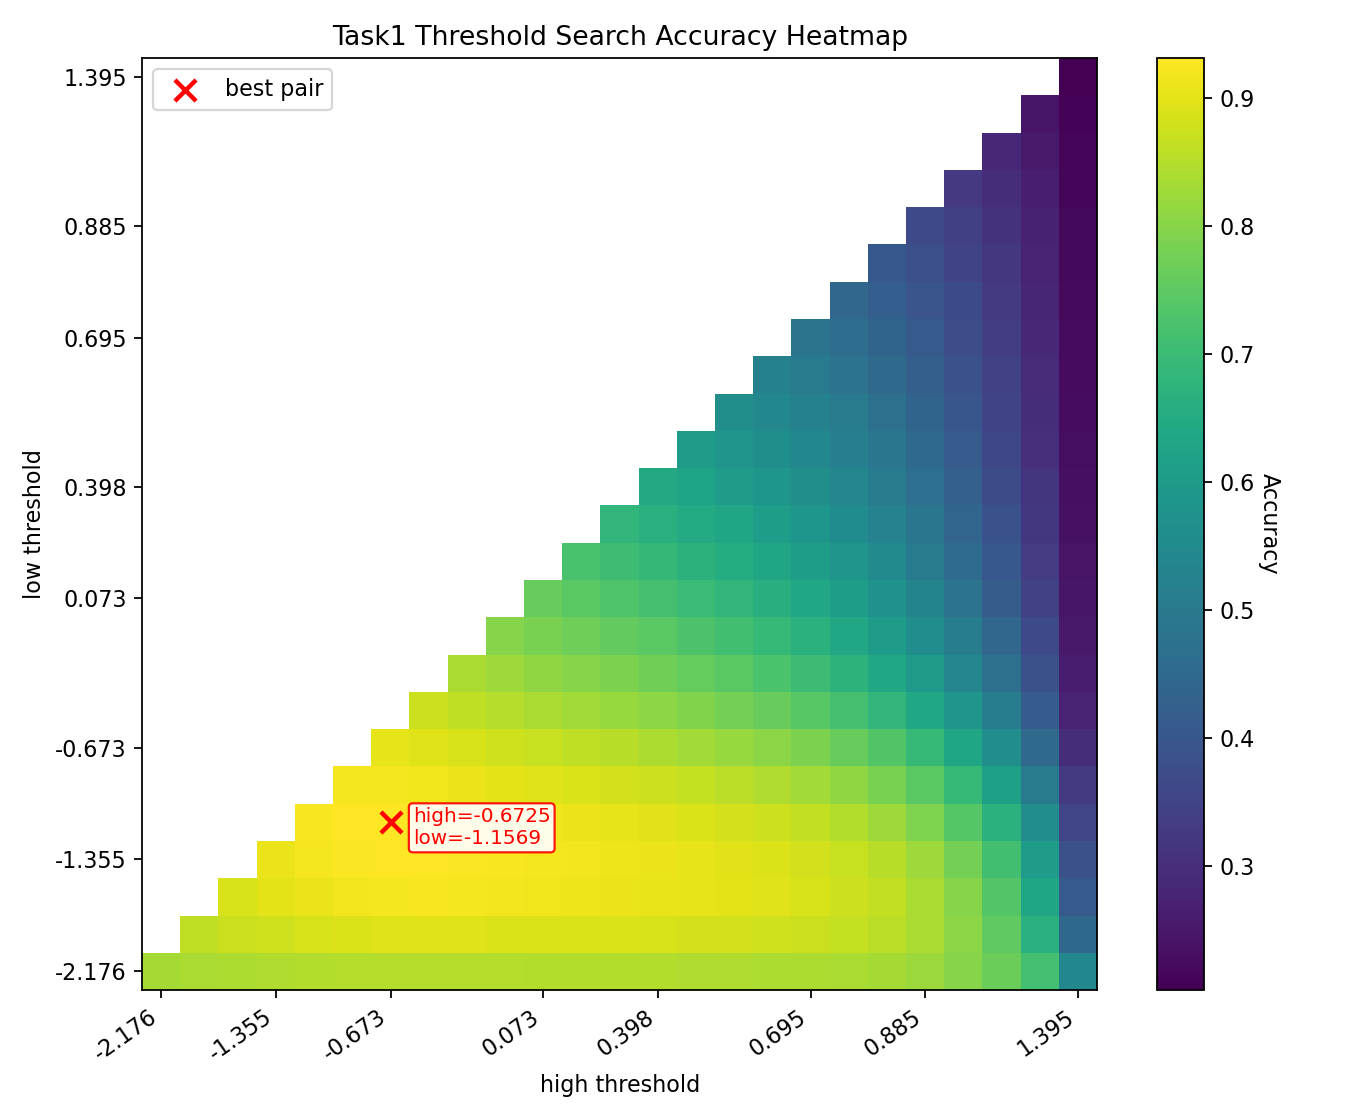
\includegraphics[width=0.88\linewidth]{figs/task1_threshold_heatmap.png}
  \captionof{figure}{Task1（能量特征、无窗函数）双阈值网格搜索图，用于选择最优 $\tau_h,\tau_l$。}
  \label{fig:task1-threshold-heatmap}
\end{center}

\begin{center}
  \centering
  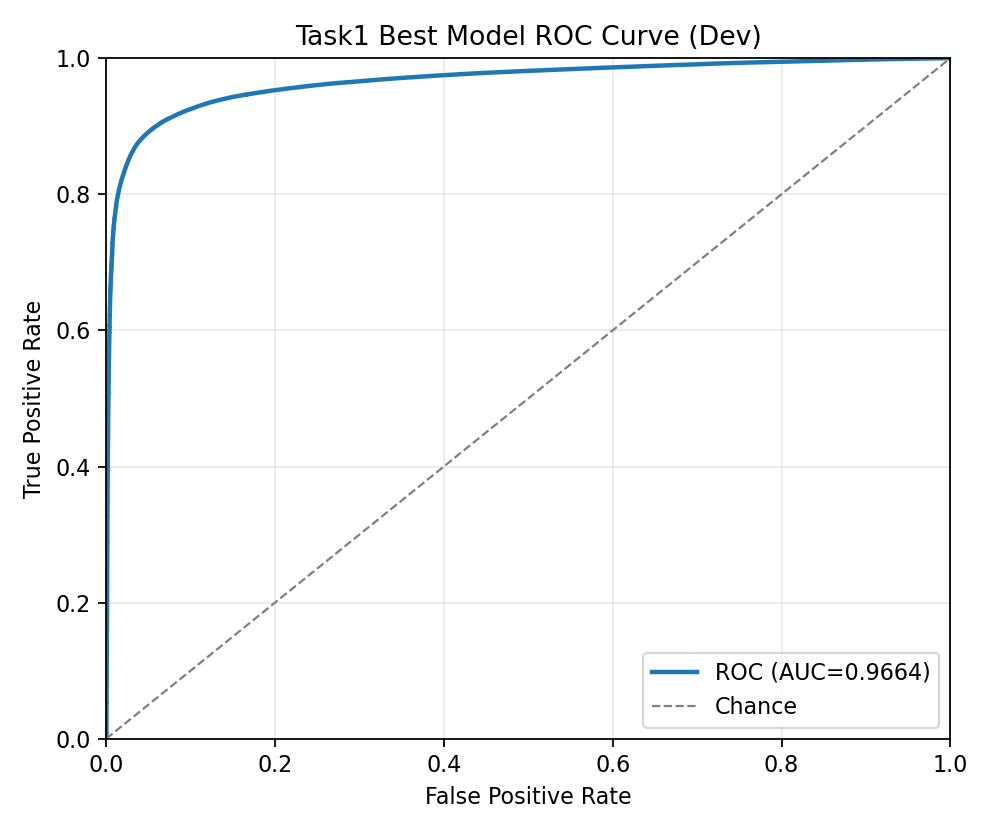
\includegraphics[width=0.88\linewidth]{figs/task1_energy_roc.png}
  \captionof{figure}{Task1（能量特征、无窗函数）$\mathcal{D}_{\text{dev}}$ ROC 曲线。}
  \label{fig:task1-roc}
\end{center}

从表~\ref{tab:task1-main} 可以看到，\textbf{能量特征在本任务中最有效}：无窗设置取得最佳
Acc/AUC/EER（95.12\%/96.64\%/8.34\%）。加入 Hamming 窗后，性能略有下降，说明当前数据条件下，
边界平滑收益不足以抵消能量判别力的损失。仅使用过零率或基频时，AUC 与 EER 明显恶化，表明二者
单独作为主判别特征不稳定。
并且可以观察到，仅使用过零率时选择出的最佳阈值接近所有帧得分的最低值，模型趋向于将绝大多数
帧判定为语音帧以获得较高准确率，此时准确率主要反映原始帧中语音帧的占比。
短时频谱特征表现介于二者之间，具备一定区分能力，但仍弱于纯能量。
此外，能量与过零率按 0.8/0.2 加权后，两种窗设置均未超过纯能量，说明本实验下过零率带来的增益有
限。综合考虑，Task1 最优配置为\textbf{能量特征 + 无窗 + 双阈值滞回判决}。且最终测试集的预测标签也是基于最优配置来进行。

\section{Task2：基于统计模型分类器和语音频域特征的语音端点检测算法}

\subsection{数据预处理及特征提取}

Task2 采用频域特征。设静态谱特征为 $\vec{u}_t \in \mathbb{R}^{K}$，其取值可为 FBank 或 MFCC。
首先以 $32$ ms 分析窗和 $8$ ms 帧移计算谱特征，再按配置拼接一阶或二阶差分：
\begin{equation}
  \vec{g}_t =
  \begin{cases}
    [\vec{u}_t;\Delta \vec{u}_t], & \text{使用一阶差分},\\
    [\vec{u}_t;\Delta \vec{u}_t;\Delta^2 \vec{u}_t], & \text{使用一阶与二阶差分}.
  \end{cases}
\end{equation}
随后对每条语音做均值方差归一化
（CMVN），并使用左右各 $1$ 帧上下文进行拼接：
\begin{equation}
  \vec{f}_t^{(2)} = [\vec{g}_{t-1};\vec{g}_{t};\vec{g}_{t+1}].
\end{equation}
因此，Task2 的最终输入既包含频谱形状信息，也包含局部动态变化信息。

\subsubsection{FBank}

\textbf{概念：}FBank 是 Mel 滤波器组上的对数能量，刻画每个感知频带内的谱能量分布。
\textbf{听觉直观：}不同 Mel 频带能量的强弱对应声音在低频、中频和高频上的明暗与厚薄；语音段通常
在若干语音相关频带上呈现稳定能量结构。\textbf{公式定义：}设第 $t$ 帧的功率谱为 $|X_t[r]|^2$，
第 $k$ 个 Mel 滤波器为 $H_k[r]$，则
\begin{equation}
  M_{t,k} = \log \left( \sum_r H_k[r]|X_t[r]|^2 + \varepsilon \right),
  \quad k=1,\dots,K.
\end{equation}

\subsubsection{MFCC}

\textbf{概念：}MFCC 是对 Mel 频带对数能量再做离散余弦变换得到的倒谱系数，用较少维度描述语音谱
包络。\textbf{听觉直观：}谱包络与音色、发音腔体形状密切相关；MFCC 去除了部分细碎谱细节，更强
调稳定的音色结构。\textbf{公式定义：}
\begin{equation}
  c_{t,q} = \sum_{k=1}^{K} M_{t,k}
  \cos\left[\frac{\pi q}{K}\left(k-\frac{1}{2}\right)\right],
  \quad q=0,\dots,K-1.
\end{equation}

\subsubsection{差分特征}

\textbf{概念：}差分特征描述相邻帧之间声学特征的动态变化，补充静态谱特征无法直接表达的时间趋
势。\textbf{听觉直观：}语音起止、音素转换和爆破音等都会带来明显的短时变化；差分项有助于捕捉这
些“变化感”。\textbf{公式定义：}设差分窗口半宽为 $R$，则一阶差分定义为
\begin{equation}
  \Delta \vec{u}_t =
  \frac{\sum_{r=1}^{R} r(\vec{u}_{t+r}-\vec{u}_{t-r})}
       {2\sum_{r=1}^{R}r^2}.
\end{equation}
二阶差分由一阶差分再次差分得到，即 $\Delta^2\vec{u}_t=\Delta(\Delta\vec{u}_t)$。

\textbf{伪代码说明：}以下代码对应 Task2 的 FBank/MFCC、差分、CMVN 与上下文拼接流程。

\begin{lstlisting}[language=python]
def extract_task2_features(waveform, feature_type, use_delta2=False):
    static = fbank_or_mfcc(waveform, win=32ms, hop=8ms, dim=K)
    delta = compute_delta(static)
    feat = concat([static, delta], axis=1)
    if use_delta2:
        delta2 = compute_delta(delta)
        feat = concat([feat, delta2], axis=1)
    feat = cmvn(feat)
    return stack_context(feat, left=1, right=1)
\end{lstlisting}

\subsection{算法描述}

\subsubsection{GMM 语音/非语音似然比模型}

GMM 方法分别对语音帧和非语音帧建模。设标准化后的特征为 $\vec{z}_t$，则训练两个类别条件密度
$p(\vec{z}_t|\mathcal{S})$ 和 $p(\vec{z}_t|\mathcal{N})$。语音类采用 $4$ 分量对角协方差高斯，非语音类采用单分量高斯。训练方式为：先用 $\mathcal{D}_{\text{tr}}$ 全部帧估计标准化器，
再按标签将标准化后的特征划分为语音帧与非语音帧，分别独立拟合两类模型，并估计语音先验
$\rho=P(y=1)$。测试时计算带先验修正的对数似然比
\begin{equation}
  \ell_t =
  \log p(\vec{z}_t|\mathcal{S})
  - \log p(\vec{z}_t|\mathcal{N})
  + \log \frac{\rho}{1-\rho},
\end{equation}
再经 Sigmoid 映射得到语音得分
\begin{equation}
  s_t = \sigma(\ell_t).
\end{equation}
得分 $s_t$ 随后交由统一的阈值判决与平滑流程得到端点检测结果。

GMM 参数 $\{\pi_m,\vec{\mu}_m,\mat{\Sigma}_m\}_{m=1}^{M}$ 使用 EM 算法估计，其中语音类与非语音
类分别独立训练。下述伪代码写作通用协方差形式；对角协方差实现时只保留 $\mat{\Sigma}_m$ 的对角元素。

\textbf{伪代码说明：}以下代码对应 GMM 的 EM 参数估计与语音/非语音似然比打分流程。

\begin{algorithm}[ht]
  \caption{GMM 的 EM 参数估计与帧级打分}
  \label{alg:gmm-em}
  \begin{algorithmic}[1]
    \Require 语音样本 $\mathcal{Z}_{\mathrm{S}}$、非语音样本 $\mathcal{Z}_{\mathrm{N}}$；混合数 $M_{\mathrm{S}}=4,M_{\mathrm{N}}=1$；待测帧 $\vec{z}_t$
    \Ensure 类别 GMM 参数 $\lambda_{\mathrm{S}},\lambda_{\mathrm{N}}$；语音得分 $s_t$
    \State $\rho\gets |\mathcal{Z}_{\mathrm{S}}|/(|\mathcal{Z}_{\mathrm{S}}|+|\mathcal{Z}_{\mathrm{N}}|)$
    \For{$c\in\{\mathrm{S},\mathrm{N}\}$}
      \State 初始化 $\lambda_c=\{\pi_m^{(c)},\vec{\mu}_m^{(c)},\mat{\Sigma}_m^{(c)}\}_{m=1}^{M_c}$
      \Repeat
        \State \textbf{E-step:} 对每个样本 $\vec{z}_i^{(c)}$ 与分量 $m$，计算责任度
        \Statex \hspace{\algorithmicindent}
        $\displaystyle
        \gamma_{im}^{(c)} =
        \frac{\pi_m^{(c)}\mathcal{N}(\vec{z}_i^{(c)};\vec{\mu}_m^{(c)},\mat{\Sigma}_m^{(c)})}
        {\sum_{j=1}^{M_c}\pi_j^{(c)}\mathcal{N}(\vec{z}_i^{(c)};\vec{\mu}_j^{(c)},\mat{\Sigma}_j^{(c)})}$
        \State \textbf{M-step:} 更新有效样本数、权重、均值和协方差
        \Statex \hspace{\algorithmicindent}
        $\displaystyle
        N_m^{(c)}=\sum_i\gamma_{im}^{(c)},\quad
        \pi_m^{(c)}=\frac{N_m^{(c)}}{N_c}$
        \Statex \hspace{\algorithmicindent}
        $\displaystyle
        \vec{\mu}_m^{(c)}=\frac{1}{N_m^{(c)}}\sum_i\gamma_{im}^{(c)}\vec{z}_i^{(c)}$
        \Statex \hspace{\algorithmicindent}
        $\displaystyle
        \mat{\Sigma}_m^{(c)}=
        \frac{1}{N_m^{(c)}}\sum_i\gamma_{im}^{(c)}
        (\vec{z}_i^{(c)}-\vec{\mu}_m^{(c)})(\vec{z}_i^{(c)}-\vec{\mu}_m^{(c)})^\top$
      \Until{对数似然收敛或达到最大迭代轮数}
    \EndFor
    \State $\ell_t\gets \log p(\vec{z}_t|\lambda_{\mathrm{S}})-\log p(\vec{z}_t|\lambda_{\mathrm{N}})$
    \Statex \hspace{\algorithmicindent}$\displaystyle\quad + \log\frac{\rho}{1-\rho}$
    \State $s_t\gets \sigma(\ell_t)$
  \end{algorithmic}
\end{algorithm}

\subsubsection{DNN 帧级分类模型}
\label{sec:dnn-model}

DNN 使用三层感知机完成逐帧二分类。输入为标准化后的频域特征，输出为
语音后验概率。设上下文半宽为 $C$，静态特征维度为 $K$；仅使用一阶差分时输入维数为
$D=(2C+1)2K$，同时使用一阶与二阶差分时输入维数为 $D=(2C+1)3K$。本实验中 $C=1$，超参数配置见第~\ref{sec:task2-config} 节。
模型输出经 Sigmoid
函数转为语音后验概率，在 $\mathcal{D}_{\text{dev}}$ 上通过阈值搜索选择最优 $\tau$，并使用长度为 $10$ 的平滑核对预测序列
做后处理。

\begin{figure}[ht]
  \centering
  \fbox{
    \parbox{0.90\columnwidth}{
      \centering
      $\vec{f}_t^{(2)}$
      $\rightarrow$
      Linear$(D,256)$
      $\rightarrow$
      ReLU
      $\rightarrow$
      Linear$(256,512)$
      $\rightarrow$
      ReLU
      $\rightarrow$
      Linear$(512,1)$
      $\rightarrow$
      Sigmoid
      $\rightarrow$
      $s_t$
    }
  }
  \caption{Task2 中 DNN 的网络结构示意图}
  \label{fig:dnn-arch}
\end{figure}

\textbf{伪代码说明：}以下代码对应 DNN 帧级分类器的前向打分流程。

\begin{lstlisting}[language=python]
def score_dnn(features, dnn):
    h = relu(linear(features, 256))
    h = relu(linear(h, 512))
    return sigmoid(linear(h, 1))
\end{lstlisting}

\subsubsection{\texorpdfstring{$\mathcal{D}_{\text{dev}}$ 阈值选择与 $\mathcal{D}_{\text{te}}$ 输出}{Ddev 阈值选择与 Dte 输出}}

Task2 在 $\mathcal{D}_{\text{tr}}$ 上训练统计模型，在 $\mathcal{D}_{\text{dev}}$ 上收集逐帧得分，并在
$[0.1,0.9]$ 区间以 $0.01$ 为步长搜索阈值，使 $\mathcal{D}_{\text{dev}}$ 帧级准确率最大。

\textbf{未知标签端点检测说明：}模型训练完成后，未知标签语音按“特征提取--模型打分--阈值判决--平滑--区间合并”的流程输出端点。

$\mathcal{D}_{\text{te}}$ 阶段复用该阈值，将二值预
测序列平滑后再转换为连续时间段输出。换言之，对未知标签语音的推理流程为：提取频域特征、执行
CMVN 与上下文拼接、送入 GMM 或 DNN 得到逐帧得分、依据阈值完成二值化、进行中值平滑、最后合并
为端点时间段。

\textbf{伪代码说明：}以下代码对应 Task2 在未知语音上的完整推理与端点输出流程。

\begin{lstlisting}[language=python]
def infer_task2(waveform, model, tau):
    features = extract_task2_features(waveform, feature_type)
    scores = model.score_frames(features)
    pred = (scores >= tau)
    pred = median_smooth(pred, kernel=10)
    return frames_to_segments(pred, win=32ms, hop=8ms)
\end{lstlisting}

\subsection{实验结果}

\subsubsection{实验指标}
Task2 使用与 Task1 相同的评测指标。模型在 $\mathcal{D}_{\text{tr}}$ 上训练，阈值选择、帧级指标和 ROC/AUC/EER 均在 $\mathcal{D}_{\text{dev}}$ 上统一计算。

\subsubsection{实验配置}
\label{sec:task2-config}

\begin{itemize}
  \item 数据划分：使用 $\mathcal{D}_{\text{tr}}$ 训练 GMM/DNN，在 $\mathcal{D}_{\text{dev}}$ 上选择阈值并统计指标，未知标签数据复用该阈值输出端点。
  \item 声学特征：采样率 $16$ kHz，帧长 $32$ ms，帧移 $8$ ms；基础特征维度 $K=40$，使用 CMVN、左右各 $1$ 帧上下文，并比较 FBank/MFCC 及其差分组合，特征名中的
$+\Delta$ 与 $+\Delta^2$ 分别表示拼接一阶与二阶差分。
  \item GMM 配置：语音类使用 $4$ 个对角协方差高斯分量，非语音类使用单个高斯分量；模型输入先由训练集估计标准化器。
  \item DNN 配置：Network1 为两层隐藏层 MLP（$256/512$）；批量实验配置中的 Network2 在隐藏层后加入 BatchNorm 与 Dropout。训练使用 Adam、学习率 $10^{-3}$、权重衰减 $10^{-5}$、batch size 为 $5210$，并采用 Focal Loss（$\alpha=0.25,\gamma=2.0$）。消融实验训练 $10$ 轮，最终配置训练 $40$ 轮。
  \item 判决与后处理：阈值在 $[0.1,0.9]$ 内以 $0.01$ 步长搜索，二值预测后采用长度为 $10$ 的平滑核。
\end{itemize}

\subsubsection{结果分析}

\textbf{GMM 结果：}GMM 中语音类使用 $4$ 个对角协方差高斯分量，非语音类使用单个高斯分量。

\begin{center}
  \scriptsize
  \setlength{\tabcolsep}{2.4pt}
  \captionof{table}{Task2 GMM $\mathcal{D}_{\text{dev}}$ 结果（\%）}
  \label{tab:task2-gmm}
  \resizebox{\columnwidth}{!}{%
    \begin{tabular}{lrrrrrrrr}
      \toprule
      特征 & Acc & Prec & Rec & $F_1$ & FAR & FRR & AUC & EER \\
      \midrule
      FBank & 93.11 & 98.18 & 92.83 & 95.43 & 7.68 & 7.17 & 96.08 & 7.35 \\
      FBank+$\Delta$ & 94.53 & \best{99.09} & 93.99 & 96.47 & \best{3.84} & 6.01 & 97.10 & 4.98 \\
      FBank+$\Delta+\Delta^2$ & 95.61 & 98.85 & 95.61 & 97.20 & 4.95 & 4.39 & 96.99 & \best{4.66} \\
      MFCC & 93.31 & 97.70 & 93.86 & 95.74 & 9.86 & 6.14 & 96.92 & 7.18 \\
      MFCC+$\Delta$ & \best{96.07} & 98.22 & \best{96.86} & \best{97.54} & 7.84 & \best{3.14} & \best{97.91} & 4.94 \\
      \bottomrule
    \end{tabular}%
  }
\end{center}

\begin{center}
  \centering
  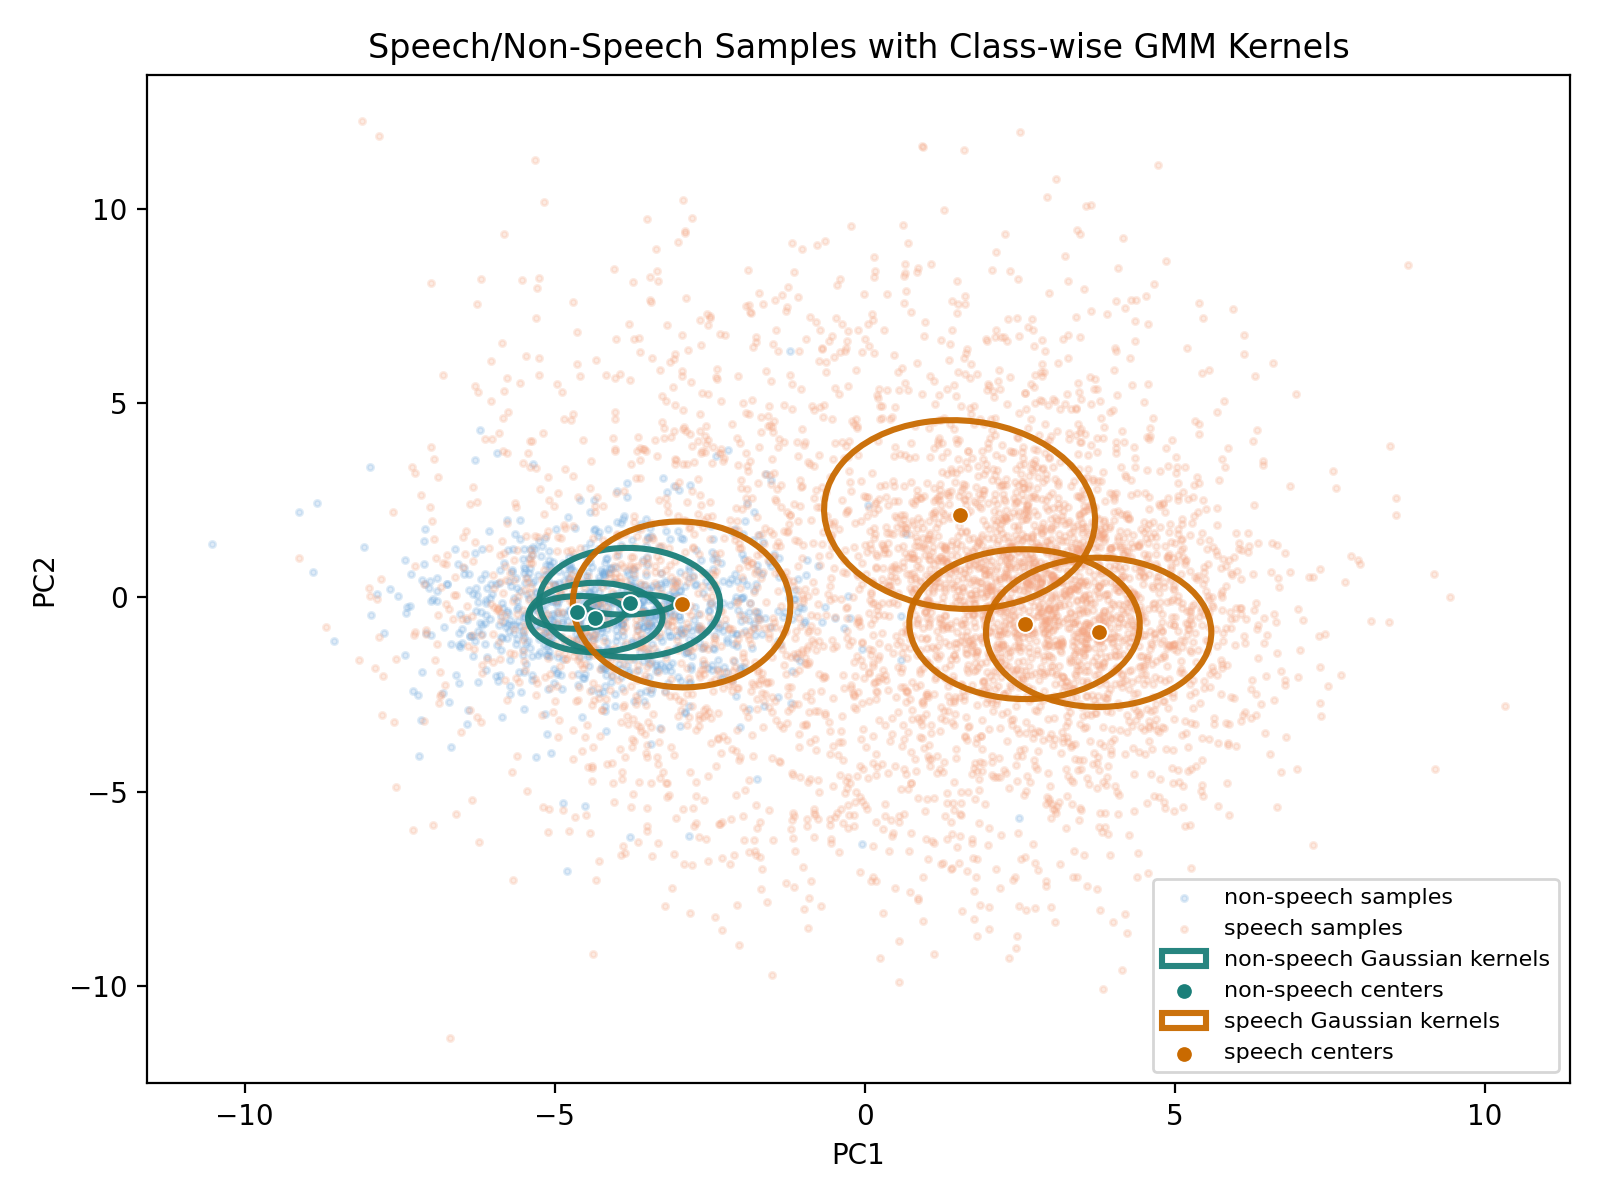
\includegraphics[width=0.88\linewidth]{figs/task2_gmm_speech_components.png}
  \captionof{figure}{GMM 最优配置（MFCC+$\Delta$）的语音类混合分量诊断图。}
  \label{fig:task2-gmm-components}
\end{center}

\begin{center}
  \centering
  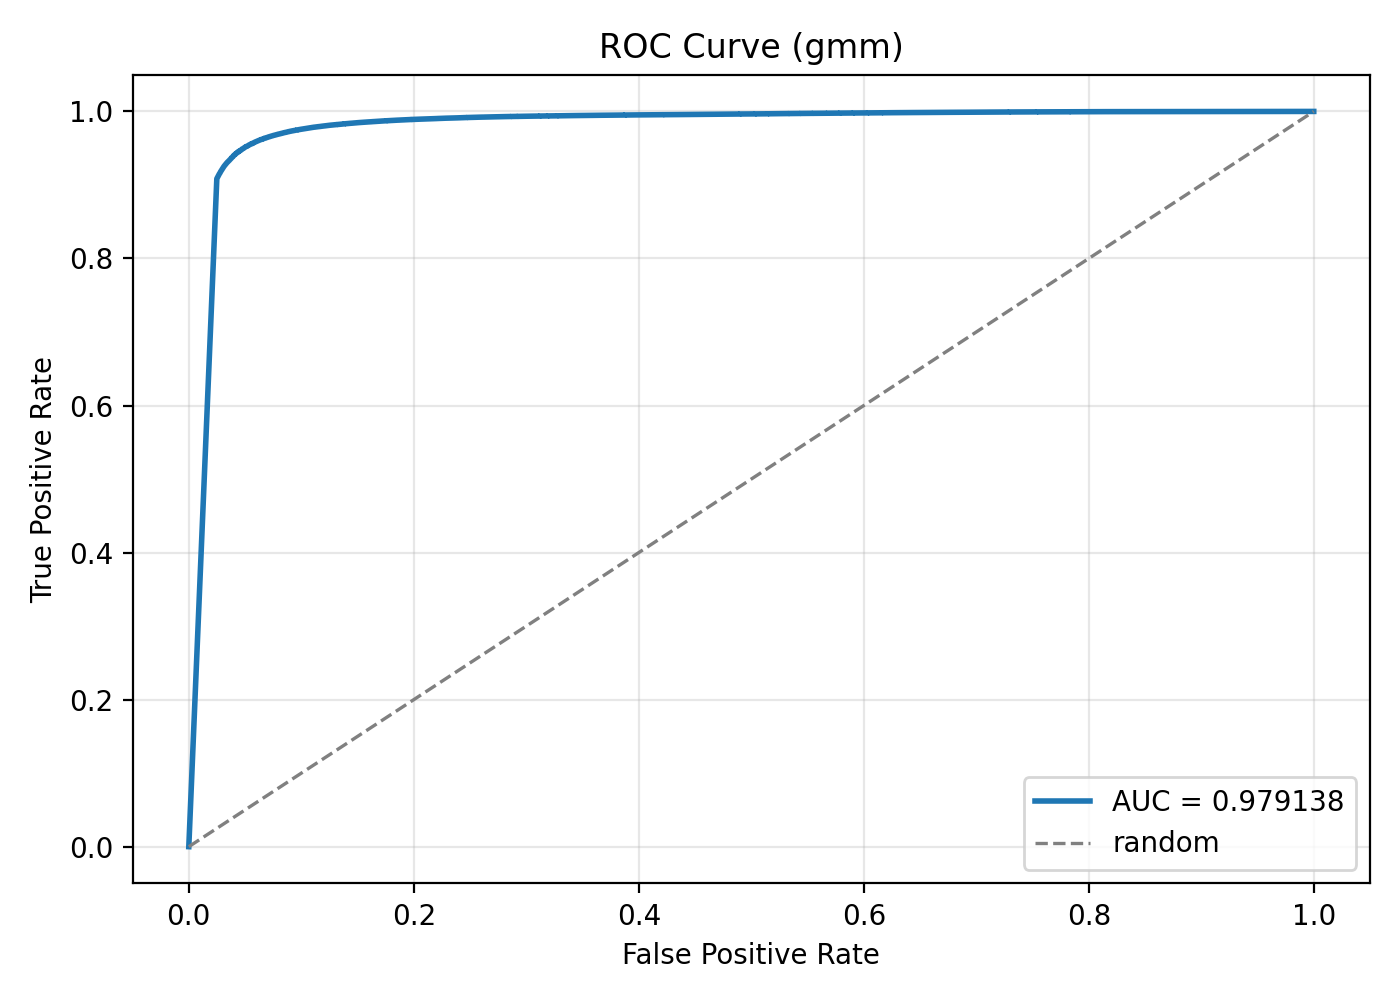
\includegraphics[width=0.88\linewidth]{figs/task2_gmm_roc.png}
  \captionof{figure}{GMM 最优配置（MFCC+$\Delta$）的 $\mathcal{D}_{\text{dev}}$ ROC 曲线。}
  \label{fig:task2-gmm-roc}
\end{center}


从表~\ref{tab:task2-gmm} 可以看到，MFCC+$\Delta$ 在 Acc、Recall、$F_1$、FRR 与 AUC 上最优，
是 GMM 的综合最佳配置。FBank 保留更细粒度的滤波器组能量，在高维条件下可能增加 GMM 的建模难度；
MFCC 主要保留谱包络信息，表示更紧凑，因此更符合 GMM 的高斯建模假设。


\textbf{DNN 结果：}DNN 对比 Network1 与 Network2 两种网络配置。受训练时间限制，消融实验均采用较轻量的训练设置。
后续再对简单配置下表现较好的模型进行规模更大的实验。

\begin{center}
  \scriptsize
  \setlength{\tabcolsep}{2.4pt}
  \captionof{table}{Task2 DNN $\mathcal{D}_{\text{dev}}$ 10 轮训练结果（\%）}
  \label{tab:task2-dnn}
  \resizebox{\columnwidth}{!}{%
    \begin{tabular}{llrrrrrrrr}
      \toprule
      网络 & 特征 & Acc & Prec & Rec & $F_1$ & FAR & FRR & AUC & EER \\
      \midrule
      Network1 & FBank & 96.93 & 98.26 & 97.70 & 97.98 & 7.71 & 2.30 & 99.13 & 3.72 \\
      Network1 & FBank+$\Delta$ & 98.05 & 98.72 & 98.85 & 98.78 & 5.74 & 1.15 & 99.61 & 2.59 \\
      Network1 & FBank+$\Delta+\Delta^2$ & \best{98.14} & \best{98.78} & 98.89 & \best{98.84} & \best{5.44} & 1.11 & \best{99.63} & \best{2.47} \\
      Network1 & MFCC & 96.59 & 98.26 & 97.26 & 97.76 & 7.67 & 2.74 & 98.93 & 4.02 \\
      Network1 & MFCC+$\Delta$ & 97.92 & 98.63 & 98.75 & 98.69 & 6.12 & 1.25 & 99.52 & 2.75 \\
      Network2 & FBank & 96.92 & 98.19 & 97.76 & 97.98 & 8.04 & 2.24 & 99.13 & 3.74 \\
      Network2 & FBank+$\Delta$ & 98.04 & 98.66 & \best{98.90} & 98.78 & 6.01 & \best{1.10} & 99.60 & 2.61 \\
      Network2 & FBank+$\Delta+\Delta^2$ & 98.11 & 98.75 & 98.89 & 98.82 & 5.57 & 1.11 & 99.63 & 2.47 \\
      Network2 & MFCC & 96.61 & 98.26 & 97.29 & 97.77 & 7.67 & 2.71 & 98.95 & 3.98 \\
      Network2 & MFCC+$\Delta$ & 97.97 & 98.62 & 98.85 & 98.73 & 6.18 & 1.15 & 99.55 & 2.66 \\
      \bottomrule
    \end{tabular}%
  }
\end{center}

其中，Network1 为基础 MLP，结构如上文所述（第~\ref{sec:dnn-model} 节）；Network2 为批量实验配置中的
MLP 变体，在 Network1 的隐藏层后加入 BatchNorm 与 Dropout，用于增强训练稳定性并缓解过拟合。

在 10 轮训练设置下，Network1 + FBank+$\Delta+\Delta^2$ 取得较优整体性能。进一步延长训练至
$40$ 轮，并保持左右各 $1$ 帧上下文后，本实验对两个较强的 Network1 配置进行单独比较，结果如表~\ref{tab:task2-dnn-40}。
最终测试集的预测标签也基于最佳模型配置生成。


\begin{center}
  \scriptsize
  \setlength{\tabcolsep}{2.4pt}
  \captionof{table}{Task2 DNN $\mathcal{D}_{\text{dev}}$ 40 轮训练结果（\%）}
  \label{tab:task2-dnn-40}
  \resizebox{\columnwidth}{!}{%
    \begin{tabular}{llrrrrrrrr}
      \toprule
      网络 & 特征 & Acc & Prec & Rec & $F_1$ & FAR & FRR & AUC & EER \\
      \midrule
      Network1 & FBank+$\Delta$ & 98.07 & 98.73 & 98.84 & 98.79 & 5.65 & 1.16 & 99.61 & 2.57 \\
      Network1 & FBank+$\Delta+\Delta^2$ & \best{98.16} & \best{98.78} & \best{98.90} & \best{98.84} & \best{5.43} & \best{1.10} & \best{99.63} & \best{2.48} \\
      \bottomrule
    \end{tabular}%
  }
\end{center}

\begin{center}
  \centering
  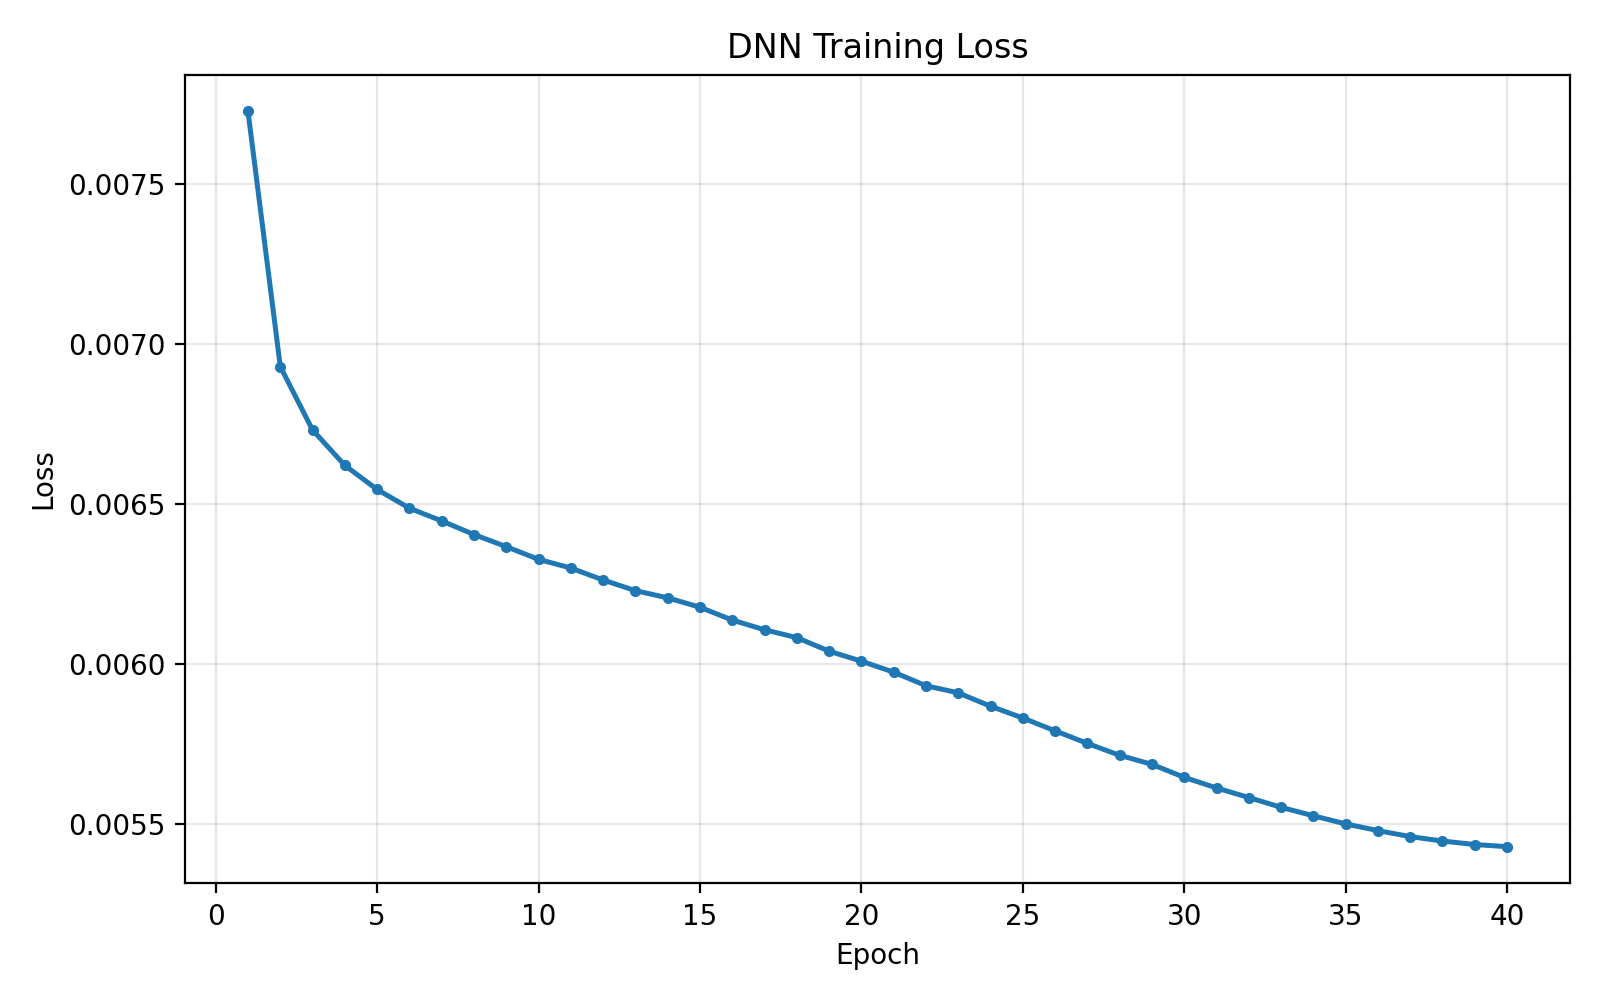
\includegraphics[width=0.88\linewidth]{figs/task2_dnn_train_loss.png}
  \captionof{figure}{DNN 最终配置（Network1，FBank+$\Delta+\Delta^2$，40 轮训练）的训练损失曲线。}
  \label{fig:task2-dnn-loss}
\end{center}

\begin{center}
  \centering
  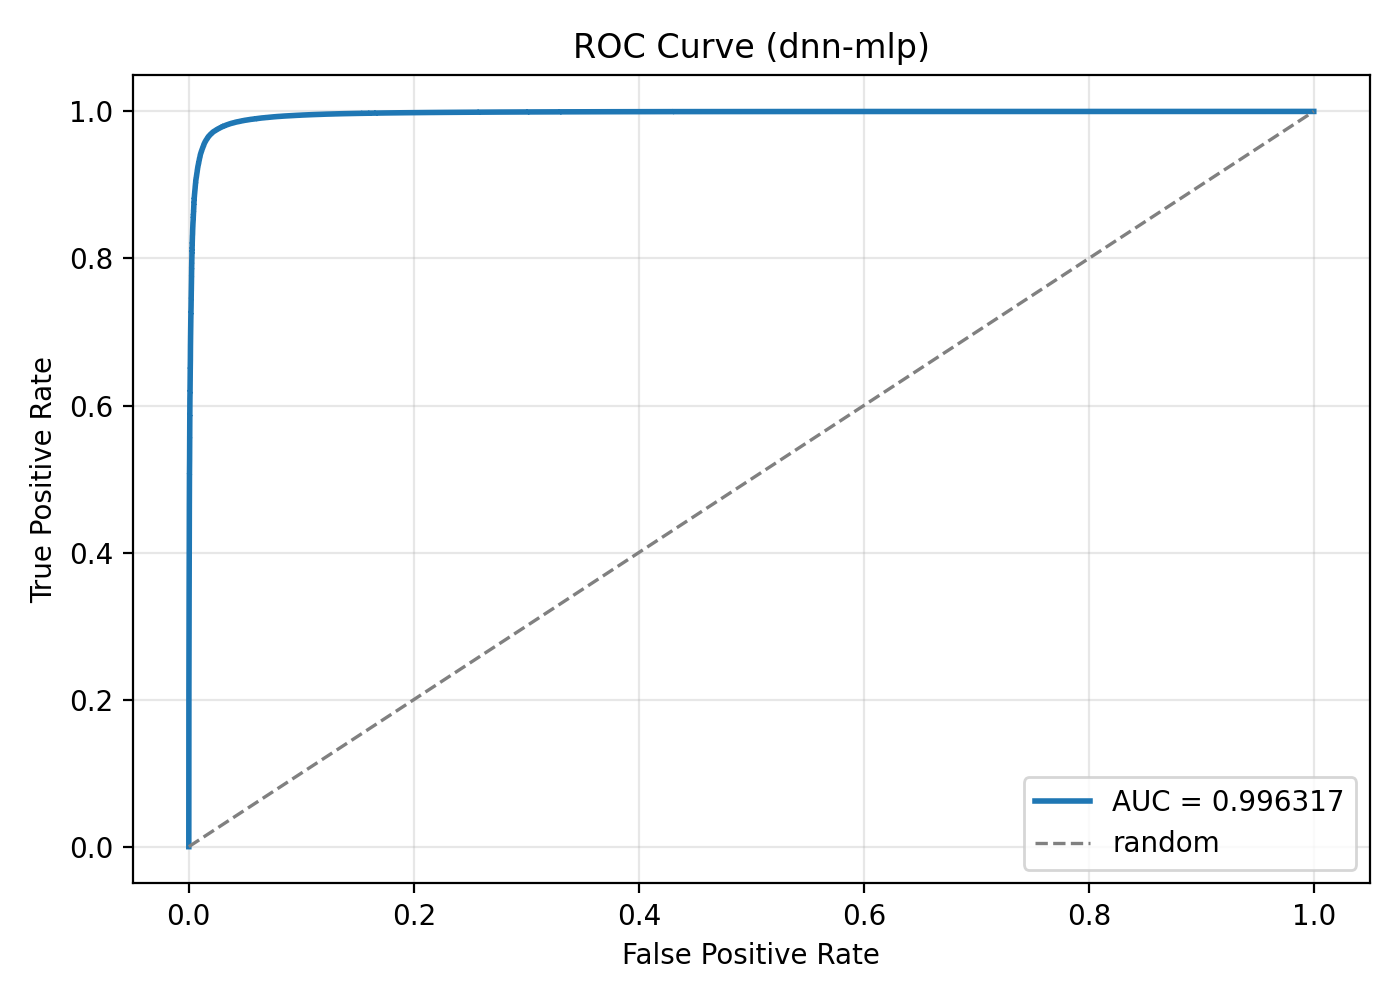
\includegraphics[width=0.88\linewidth]{figs/task2_dnn_roc.png}
  \captionof{figure}{DNN 最终配置（Network1，FBank+$\Delta+\Delta^2$，40 轮训练）的 $\mathcal{D}_{\text{dev}}$ ROC 曲线。}
  \label{fig:task2-dnn-roc}
\end{center}

从表~\ref{tab:task2-dnn-40} 可以看到，新 40 轮配置在 Acc、Recall、$F_1$、FAR、FRR、AUC 与
EER 上均优于旧 40 轮配置，因此本实验最终 DNN 配置采用 Network1 + FBank+$\Delta+\Delta^2$。与
GMM 相比，DNN 在整体准确率和 AUC 上均有明显提升，说明判别式模型能更充分利用频域动态特征。加入差分特征和
上下文帧信息能够显著提高模型预测准确率，说明端点检测需要利用相邻帧的时序连续性辅助判断。



\end{document}

% \section{基于线性分类器和语音短时能量的简单语音端点检测算法}

% \subsection{数据预处理及特征提取}

% 本节介绍任务1中你对输入数据进行了哪些预处理步骤，提取了什么特征。对每种预处理步骤，请简要
% 介绍该步骤的效果或功能；对每种特征，请简要介绍该特征的定义和/或该特征对人耳听觉造成的直观
% 感受。\textbf{写作完成后，请删除本段。}

% \subsection{算法描述}

% 请描述你的语音端点检测算法。若不止一种，可继续分节。请尽可能使用伪代码描述。如有必要，可以
% 贴出少量程序代码。\textbf{写作完成后，请删除本段。}

% \subsection{实验结果}

% 请使用表格等形式给出你的算法在开发集上的性能表现。\textbf{写作完成后，请删除本段。}

% \section{基于统计模型分类器和语音频域特征的语音端点检测算法}

% \subsection{数据预处理及特征提取}

% 本节介绍任务2中你对输入数据进行了哪些预处理步骤，提取了什么特征。对每种预处理步骤，请简要
% 介绍该步骤的效果或功能；对每种特征，请简要介绍该特征的定义。\textbf{写作完成后，请删除本段
% 。}

% \subsection{算法描述}

% 请描述你的语音端点检测算法。若不止一种，可继续分节。若你使用GMM，请描述其具体参数设置及训
% 练方式；若你使用NN，请描述其结构、具体参数设置及训练方式。此外，还请描述模型训练完成后，如
% 何使用模型对未知标签的数据进行端点检测。请尽可能使用伪代码描述。如有必要，可以贴出少量程序
% 代码。\textbf{写作完成后，请删除本段。}

% \subsection{实验结果}

% 请使用表格等形式给出你的算法在开发集上的性能表现。\textbf{写作完成后，请删除本段。}
